	\documentclass[11pt]{article}
\usepackage[UTF8]{ctex}
\usepackage{picinpar,graphicx,bm}
\usepackage{booktabs}
\usepackage{diagbox}
\usepackage{float}
\usepackage{setspace}
\newcommand{\upcite}[1]{\textsuperscript{\textsuperscript{\cite{#1}}}}

% used to demo bracket for array
\usepackage{amsmath}

\usepackage{listings}
\usepackage{xcolor}
% 定义可能使用到的颜色
\definecolor{CPPLight}  {HTML} {686868}
\definecolor{CPPSteel}  {HTML} {888888}
\definecolor{CPPDark}   {HTML} {262626}
\definecolor{CPPBlue}   {HTML} {4172A3}
\definecolor{CPPGreen}  {HTML} {487818}
\definecolor{CPPBrown}  {HTML} {A07040}
\definecolor{CPPRed}    {HTML} {AD4D3A}
\definecolor{CPPViolet} {HTML} {7040A0}
\definecolor{CPPGray}  {HTML} {B8B8B8}
\lstset{
    columns=fixed,    
   % numbers=left,                                        % 在左侧显示行号
    frame=none,                                          % 不显示背景边框
    backgroundcolor=\color[RGB]{245,245,244},            % 设定背景颜色
    keywordstyle=\color[RGB]{40,40,255},                 % 设定关键字颜色
    numberstyle=\footnotesize\color{darkgray},           % 设定行号格式
    commentstyle=\it\color[RGB]{0,96,96},                % 设置代码注释的格式
    stringstyle=\rmfamily\slshape\color[RGB]{128,0,0},   % 设置字符串格式
    showstringspaces=false,                              % 不显示字符串中的空格
    language=c++,                                        % 设置语言
    morekeywords={alignas,continute,friend,register,true,alignof,decltype,goto,
    reinterpret_cast,try,asm,defult,if,return,typedef,auto,delete,inline,short,
    typeid,bool,do,int,signed,typename,break,double,long,sizeof,union,case,
    dynamic_cast,mutable,static,unsigned,catch,else,namespace,static_assert,using,
    char,enum,new,static_cast,virtual,char16_t,char32_t,explict,noexcept,struct,
    void,export,nullptr,switch,volatile,class,extern,operator,template,wchar_t,
    const,false,private,this,while,constexpr,float,protected,thread_local,
    const_cast,for,public,throw,std,size_t,__global__,__device__,__host__},
    emph={map,set,multimap,multiset,unordered_map,unordered_set,
    unordered_multiset,unordered_multimap,vector,string,list,deque,
    array,stack,forwared_list,iostream,memory,shared_ptr,unique_ptr,
    random,bitset,ostream,istream,cout,cin,endl,move,default_random_engine,
    uniform_int_distribution,iterator,algorithm,functional,bing,numeric,},
    emphstyle=\color{CPPViolet}, 
    frame=shadowbox,
    basicstyle=\footnotesize\ttfamily,
    tabsize=4,
}


%layout
\usepackage{calc} 
\setlength\textwidth{7in} 
\setlength\textheight{9in} 
\setlength\oddsidemargin{(\paperwidth-\textwidth)/2 - 1in}
\setlength\topmargin{(\paperheight-\textheight -\headheight-\headsep-\footskip)/2 - 1.5in}


\title{应用几何造型 \hspace{2pt}\hspace{2pt} \begin{large}----- \hspace{2pt}  流形的表示\end{large} }
\author{11821095 葛林林}
\begin{document}
\maketitle
\section{引言}
对于流形的表示始终是几何造型领域非常重要的研究方向。流形是指空间上的每一点都可以拓扑同胚与一个圆盘,例如圆柱面、圆锥面都可以算作流形,而存在相交的表面则为非流形。

流形的表示有许多的研究方向:(1) Sharp Feature的处理;(2) 高度详细的表面模型;(3)
\section{流形表示方法的介绍}
\subsection{参数曲面}
参数曲面是流形表示中最重要的一大类,参数曲面拥有易于绘制的优点,然而这种方法需要相对应的数据结构来表现连通性以及提高在图形渲染、碰撞检测等应用中的灵活性\upcite{ADFs}。除此之外,参数曲面不是直接的表示对象的内部或者外部使得很难进行bool操作。
\subsubsection{线框表示法} 其优点是表示简单,缺点是表示的时候存在歧义。
\subsubsection{多边形表示法}多边形表示法由顶点、边和面组成,能够有效的解决线框表示法存在的歧义问题。多边形表示法被广泛用于工业设计的模型存储当中,例如PLY、Obj文件格式都是基于多边形表示法。如下图所示是线框表示法的示意图。
\begin{figure}[H]
\begin{center}
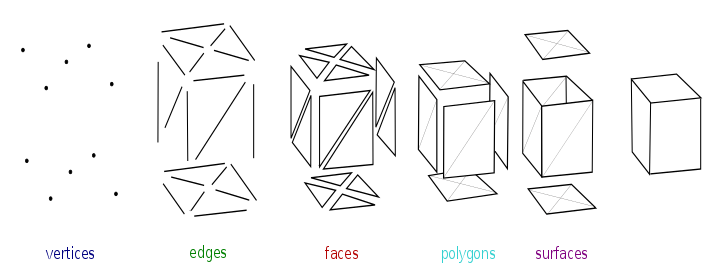
\includegraphics[scale=0.5]{polygon.png}
\end{center}
\caption{线框表示法示意图}
\end{figure}
\subsubsection{Bezier表示法}该方法建立在Berstein基函数的基础上。优点:(1)只需要很少的点来表示曲面;
(2)很容易控制形状。缺点:(1)Bernstein基是全局的;(2)次数是固定的(等于控制控制点的个数);(3)为了提高灵活性需要很高的次数;(4)很难保证光滑性;(5)很难与线求交;(6)很难与透射投影算法进行结合。
\begin{figure}[H]
\begin{center}
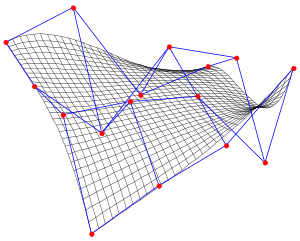
\includegraphics[scale=0.7]{bezier_surface1.png}
\end{center}
\end{figure}


\subsubsection{B-spline表示法\upcite{b-spline0}}该方法在上世纪40年代由Isaac Jacob Schoenberg提出,它建立在B-spline基函数的基础上,通过控制顶点和阶次来控制曲面的形状。优点:构造的曲面$C^0,C^1$连续。
\begin{figure}[H]
\begin{center}
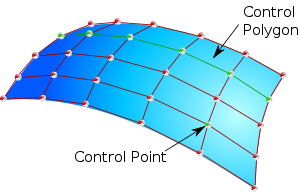
\includegraphics[scale=0.7]{b-spline-surface1.png}
\end{center}
\caption{B-spline曲面示意图}
\end{figure}

\subsubsection{NURBS表示法}


\subsection{细分曲面} 
\bm{发展历程} 
\begin{table}[H]
\begin{tabular}{lp{16cm}}
1978年&由Edwin Catmull 和Jim Clark首次提出,随后Catmull和Clark\upcite{subdivision1},Doo和Sabin\upcite{subdivision2},Loop\upcite{subdivision3}分别进行了细化。\\
1994年& Hoppe等人\upcite{subdivision_ex1}将细分曲面应用到sharp feature的处理上。\\
1998年&DeRose等人\upcite{subdivision_ex2}在细分曲面上提出了subdivision mask的概念,并在此基础上提出了细分曲面的标量场。\\
2001年 & Displaced Subdivision Surface\upcite{DSS}由Aaron Lee、Henry Moreton和Hugues Hoppe在2001年的siggraph会议上提出,它便于几何压缩、编辑、动画制作,并且在图形渲染方面拥有很好的可扩展性和自适应性。\\
\end{tabular}
\end{table}
细分曲面是通过从一个指定的粗糙的分段多边形网格出发,通过递归不断的将每个多边形切分成更小的面片从而逼近一个光滑的曲面。
\begin{table}[H]
\begin{tabular}{lp{16cm}}
\bm{优点}&它不需要控制点的约束而能够表示任意拓扑类型。\\
\bm{缺点\upcite{ADFs}}&(1)与参数曲面类似,它依赖于大量的数据结构;
(2)需要处理特殊点;
(3)难于控制和编辑。\\
\end{tabular}
\end{table}

细分曲面经常被用于三维动画角色的原型设计,如下图所示是《Geri's Game》中利用细分曲面得到的人物模型。
\begin{figure}[H]
\begin{center}
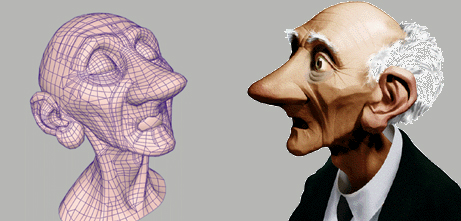
\includegraphics[scale=0.8]{Geri_s_Game.png}
\end{center}
\caption{Geri's Game中人物的细分曲面模型}
\end{figure}

\subsection{隐式曲面} 
优点:
(1)易于区分物体的内部和外部;
(2)易于对象之间的混合。
缺点:
(1)进行求交运算非常耗时;
(2)对于任意的物体很难找到对应隐式曲面

\subsection{小波表示法}
\subsection{距离场表示法} 优点是能够很好的显示表面的细节。

\subsection{Normal Meshes}


\subsection{Semi-regular Meshes}

\subsection{Surfels}

\subsection{Wavelets}

\subsection{Adaptive Sampled Distance Fields}


\subsection{Multi-resolution Triangulation}

\section{应用领域}

\section{当前存在的问题}


\begin{thebibliography}{1}
\bibitem{b-spline0} Knott, Gary D. Interpolating cubic splines. Vol. 18. Springer Science \& Business Media, 2012.

\bibitem{subdivision1}Catmull, Edwin, and James Clark. "Recursively generated B-spline surfaces on arbitrary topological meshes." Computer-aided design 10.6 (1978): 350-355.

\bibitem{subdivision2} Doo, Daniel, and Malcolm Sabin. "Behaviour of recursive division surfaces near extraordinary points." Computer-Aided Design 10.6 (1978): 356-360.

\bibitem{subdivision3} Loop, Charles. "Smooth subdivision surfaces based on triangles." Master's thesis, University of Utah, Department of Mathematics (1987).

\bibitem{subdivision_ex1} Hoppe, Hugues, et al. "Piecewise smooth surface reconstruction." Proceedings of the 21st annual conference on Computer graphics and interactive techniques. ACM, 1994.

\bibitem{subdivision_ex2} DeRose, Tony, Michael Kass, and Tien Truong. "Subdivision surfaces in character animation." Proceedings of the 25th annual conference on Computer graphics and interactive techniques. ACM, 1998.

\bibitem{DSS} Lee, Aaron, Henry Moreton, and Hugues Hoppe. "Displaced subdivision surfaces." Proceedings of the 27th annual conference on Computer graphics and interactive techniques. ACM Press/Addison-Wesley Publishing Co., 2000.

\bibitem{normal-meshes} Guskov, Igor, et al. "Normal meshes." Proceedings of the 27th annual conference on Computer graphics and interactive techniques. ACM Press/Addison-Wesley Publishing Co., 2000.

\bibitem{surface-splatting}Zwicker, Matthias, et al. "Surface splatting." Proceedings of the 28th annual conference on Computer graphics and interactive techniques. ACM, 2001.

\bibitem{} Pauly, Mark, and Markus Gross. "Spectral processing of point-sampled geometry." Proceedings of the 28th annual conference on Computer graphics and interactive techniques. ACM, 2001.

\bibitem{ADFs} Frisken, Sarah F., et al. "Adaptively sampled distance fields: A general representation of shape for computer graphics." Proceedings of the 27th annual conference on Computer graphics and interactive techniques. ACM Press/Addison-Wesley Publishing Co., 2000.

\end{thebibliography}



\end{document}